\documentclass[12pt,a4paper,twocolumn]{article}
% The following LaTeX packages must be installed on your machine: amsmath, authblk, bm, booktabs, caption, dcolumn, fancyhdr, geometry, graphicx, hyperref, latexsym, natbib
\input{151.dat}
\usepackage{gensymb}
\usepackage{amsthm}
\usepackage{float}
\usepackage{siunitx}
\usepackage{amssymb}
\usepackage{float}
\usepackage{enumerate}
\usepackage{listings}
\usepackage{mathtools}
\PassOptionsToPackage{hyphens}{url}\usepackage{hyperref}
\usepackage[none]{hyphenat}
\usepackage{physics}
%\renewcommand{\familydefault}{\sfdefault}


\begin{document}

\setcounter{page}{1}

\section*{PS 33: Problem 3.43}
\bigskip

\begin{enumerate}[(a)]

\item The Lorentz distribution is given by

\begin{equation}\label{eq:lorentz}
	p(x) = \frac{1}{\pi}\frac{\gamma}{(x-a)^2 + \gamma^2}
\end{equation}

Comparing it with the Gaussian distribution:

\begin{figure}[!h]
	\centering
	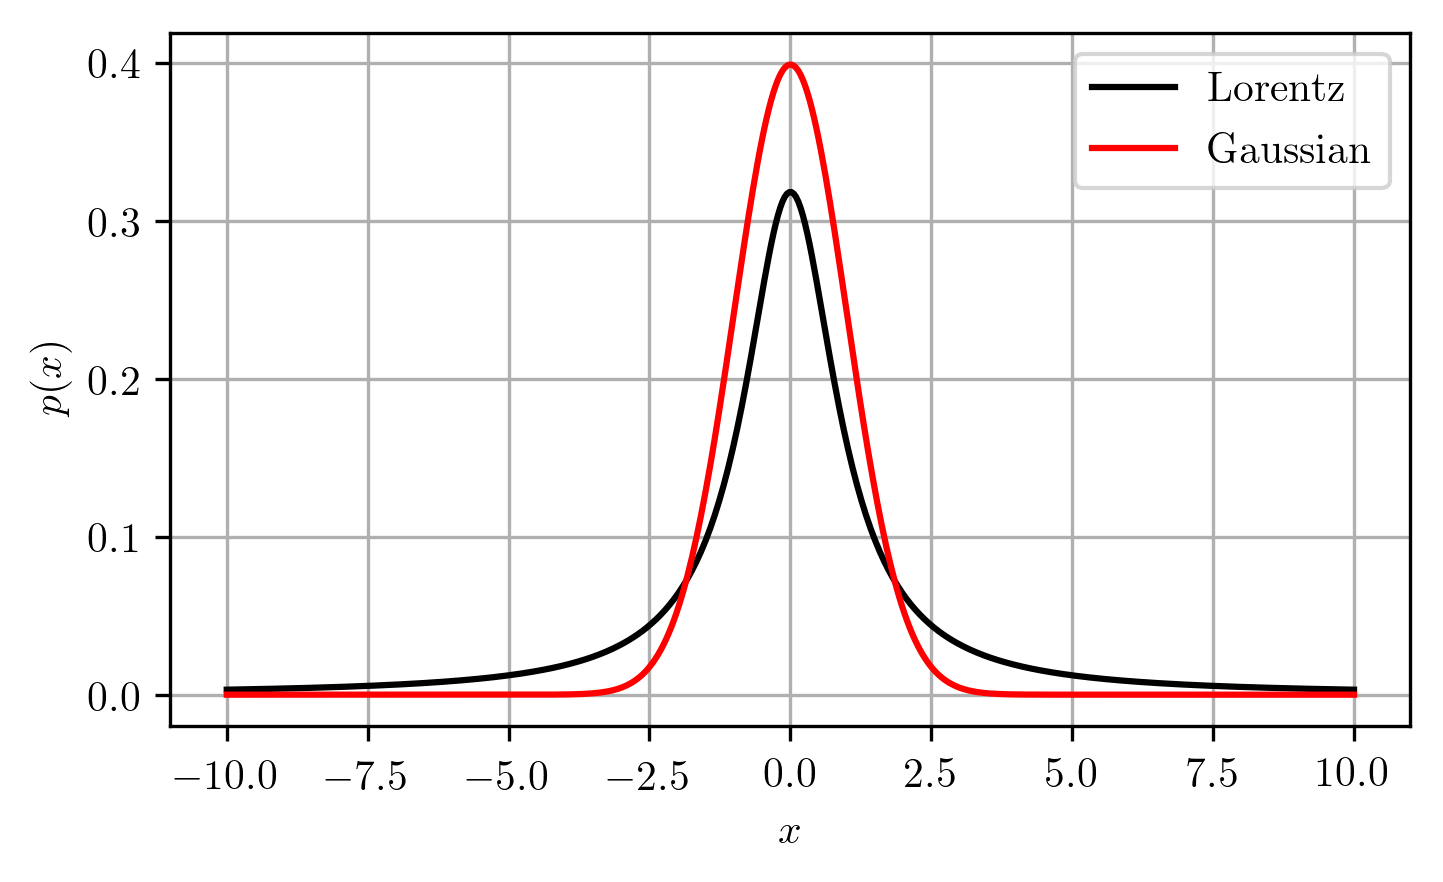
\includegraphics[width=\linewidth]{lorentz.png}
	\caption{Comparison of Lorentzian and Gaussian distributions.}
	\label{fig:compare}
\end{figure}

This shows that for the same set of parameters, the Gaussian has a higher peak, and quickly falls off and approaches zero as one moves away from the mean/central value.

\item For $a = 0$ and $\gamma = 1$, the first moment of the Lorentzian is given by

\begin{align}
	\ev{x^1} &= \int_{-\infty}^{+\infty} xp(x) \dd{x} \\
	&= \frac{1}{\pi} \int_{-\infty}^{+\infty} \frac{x}{x^2 + 1} \dd{x} \nonumber
\end{align}

Let $u \equiv x^2 + 1$, $\dd{u} \equiv 2x\dd{x}$,

\begin{align}
	\ev{x^1} &= \frac{1}{2\pi} \int_{-\infty}^{+\infty} \frac{1}{u}\dd{u} \nonumber \\
	&= \frac{1}{2\pi} \eval[\ln(u)|_{-\infty}^{+\infty} \nonumber \\
	&= \frac{1}{2\pi} \eval[\ln(x^2 + 1)|_{-\infty}^{+\infty} \nonumber \\
	&= \infty - \infty \nonumber \\
	\Aboxed{
		\ev{x} &= \mathrm{undefined}
	} \label{eq:answer-b}
\end{align}

\item The second moment is given by

\begin{equation}\label{eq:2nd-moment}
	\ev{x^2} = \frac{1}{\pi} \int_{-\infty}^{+\infty} \frac{x^2}{x^2 +1}\dd{x}
\end{equation}

By long division of the integrand,

\begin{center}
	\begin{tabular}{c|ccc}
		&&& 1 \\ \cline{2-4}
		$x^2 + 1$ & $x^2$ & $+0x+$ & $0$ \\
		& $x^2$ & $+0x+$ & $1$ \\ \cline{2-4}
		&&& $-1$
	\end{tabular}
\end{center}

From this, \eqref{eq:2nd-moment} can be rewritten as

\begin{align*}
	\ev{x^2} &= \frac{1}{\pi} \int_{-\infty}^{+\infty} 1 - \frac{1}{x^2 + 1} \dd{x} \\
	&= \frac{1}{\pi}\qty[\int_{-\infty}^{+\infty} \dd{x} - \int_{-\infty}^{+\infty} \frac{\dd{x}}{x^2 + 1}]
\end{align*}

The second term is an even function about zero, and can be rewritten as

\begin{align}
	\ev{x^2} &= \frac{1}{\pi}\qty[\int_{-\infty}^{+\infty} \dd{x} - 2\int_0^{+\infty} \frac{\dd{x}}{x^2 + 1}] \nonumber \\
	&= \frac{1}{\pi}\qty[\int_{-\infty}^{+\infty} \dd{x} - 2\eval{\arctan(x)}_0^\infty] \nonumber \\
	&= \frac{1}{\pi}\qty[\int_{-\infty}^{+\infty} \dd{x} - 2\qty(\arctan(\infty) - \arctan(0))] \nonumber \\
	&= \frac{1}{\pi}\qty[\int_{-\infty}^{+\infty} \dd{x} - 2\qty(\frac{\pi}{2} - 0)] \nonumber \\
	&= \frac{1}{\pi}\qty[\int_{-\infty}^{+\infty} \dd{x} - \pi] \nonumber \\
	&= \frac{1}{\pi} \qty[\infty - \pi] \nonumber \\
	\Aboxed{
		\ev{x^2} &= \infty
	} \label{eq:answer-c}
\end{align}

The second moment of the Lorentz distribution exists and has a value of infinity.

\end{enumerate}

\end{document}